\section{Externes Design - Android App}
\label{sec:externesdesignandroid}
Folgendes Dokument beschreibt das externe Design der Android App. Als Designgrundlage der Mockups dienen primär die in Zusammenarbeit mit cnlab Software AG festgelegten Requirements. Als Referenz stand die bestehende Symbian-App zur Verfügung. 

\subsection{Einführung}
In einem ersten Schritt wurden die Android GUI Principles\footnote{Android GUI Principles\url{http://developer.android.com/design/get-started/principles.html}, zuletzt besuch 21.03.2013}  studiert und aufgrund dieser ein Design-Konzept für die neue App erstellt.
\\

Folgend ein Beispiel einer Applikation, welche den GUI Guidelines entspricht und ähnliche Komponenten benutzt wie die zukünftige TourLiveApp.

\begin{figure}[H]
	\centering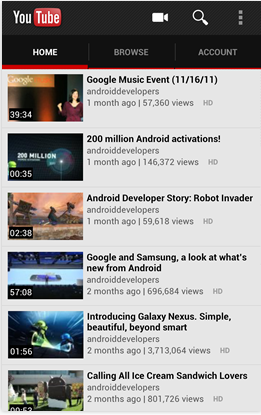
\includegraphics[width=60mm]{images/android/mockups/androidexample.png} 
	\caption{Standard Ansicht nach den Android GUI Guidelines}
\end{figure}

\subsection{Grobübersicht TourLiveApp}
Das Design der Android App gliedert sich grundsätzlich in ein Dashboard sowie 5 Informationsansichten die über Tabs erreichbar sind. Über den "Settings"-Button lassen sich Konfigurationen vornehmen sowie den About Screen anzeigen.

\begin{figure}[H]
	\centering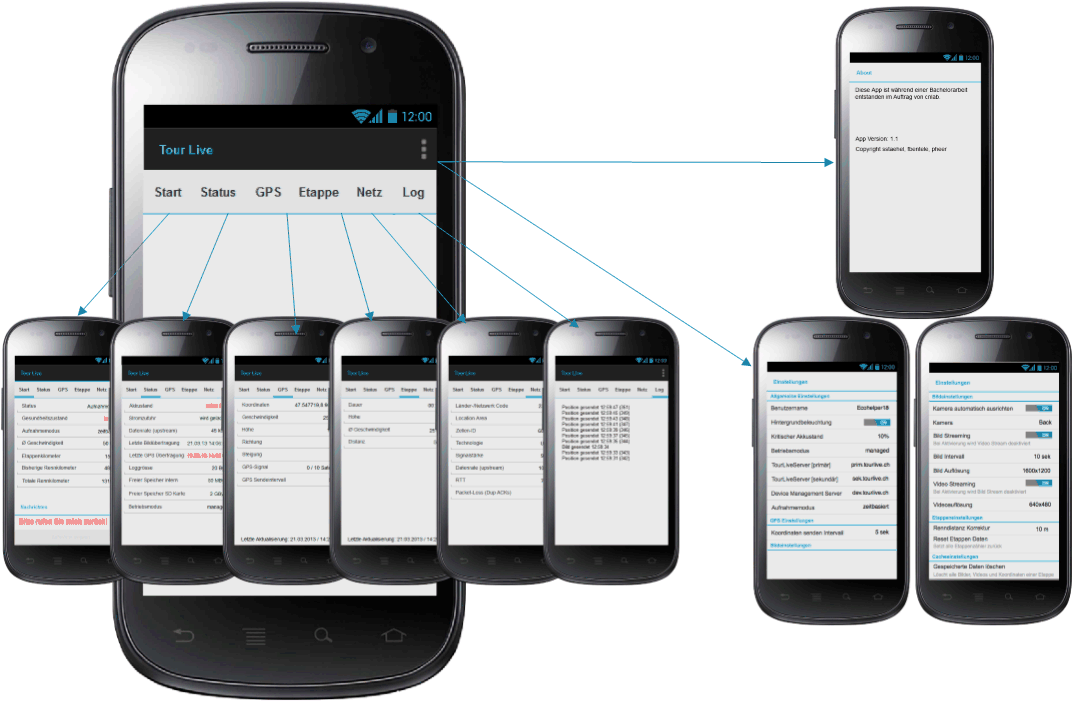
\includegraphics[width=130mm]{images/android/OverviewAndroid.png} 
	\caption{Übersicht über alle Views}
\end{figure}
 
Folgend werden alle Ansichten im Detail beschrieben. Dabei wurde auf mit Hilfe folgender Legende gearbeitet um die einzelnen Werte zu beschreiben:
* 	berechneter Wert der stets aktualisiert wird
+	Wert der aufgrund einer Messung eruiert wird (Android Service Provider)
°	App-Einstellung die angezeigt wird

\subsection{Startscreen - Ansicht}
Wird die App gestartet öffnet sich die „Start“-View. Sie dient als „Dashboard“ und gibt Informationen zum allgemeinen Zustand der App. 

\begin{longtable}{p{4cm} p{8cm}}
	\raisebox{-\totalheight}{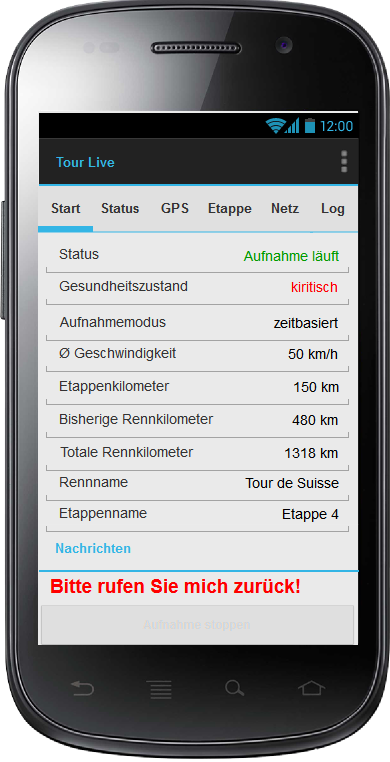
\includegraphics[width=4cm]{images/android/mockups/Start.png} }
 & \textbf{Nutzen / Zielperson }\newline

Diese View dient dazu, dem Fahrer und Beifahrer, eine Übersicht zu geben um im Falle eines Problems zu intervenieren. 
Mit Hilfe der Nachrichten kann der Systemüberwacher mit den Autoinsassen kommunizieren kann.\newline
\textbf{Erläuterung der Ansicht} \newline
\textbf{Status:} Zeigt an, ob Daten an den TourLive Server gesendet werden oder nicht \newline
\textbf{Gesundheitszustand:} Zusammenfassung der Ansicht „Status“ \newline
\textbf{Aufnahmemodus (°):} manuell, zeitbasiert, fernverwaltet, externe Stromquelle \newline
\textbf{Durchschnittsgeschwindigkeit (+):} Die Durchschnittlichegeschwindigkeit wird ermittelt, über alle bereits gemessenen Locations, anhand deren Geschwindigkeit \newline
\textbf{Etappenkilometer (*):} Die in der aktuellen Etappe zurückgelegten Kilometer \newline
\textbf{Bisherige Rennkilometer (*):} Die ganze Strecke, über mehrere Etappen verteilt, die zurückgelegt wurde. Dieser Wert wird vom TourLiveServer übermittelt. \newline
\textbf{Totale Rennkilometer (*):} Die totale Anzahl Kilometer, die in diesem Rennen zurückgelegt wird. Wird vom TourLiveServer an die App übermittelt. \newline
\textbf{Nachrichten (*):} Das Management Device Portal hat die Möglichkeit, Nachrichten via das Mobile an die Fahrer zu übermitteln. Diese werden rot dargestellt.\\

\end{longtable}



\subsection{Status - Ansicht}
Allgemeiner Zustand des Systems. Orange eingefärbte Zustände können längerfristig zu Problemen führen, rot eingefärbte Zustände sind kritisch und verhindern das einwandfreie Funktionieren des Systems. Es folgt eine Beschreibung der einzelnen Zustände: 

\begin{longtable}{p{4cm} p{8cm}}
	\raisebox{-\totalheight}{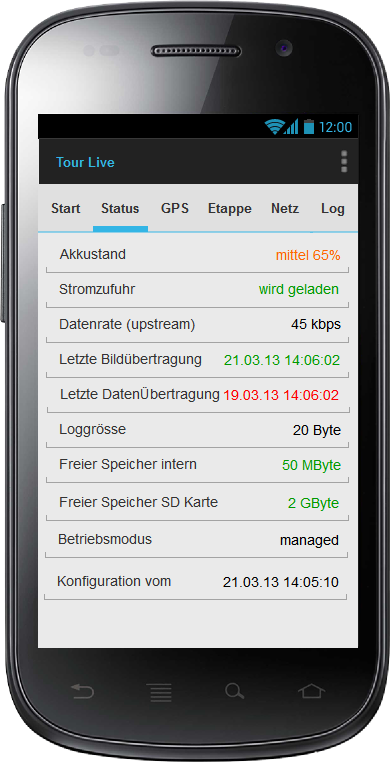
\includegraphics[width=4cm]{images/android/mockups/Status.png} }
 & \textbf{Nutzen / Zielperson }\newline

Zielperson ist auch hier der Laie (Fahrer / Beifahrer der auf einen Blick sehen möchte ob die App korrekt funktioniert.  Aus diesem Grund werden problematische Werte orange und kritische Werte rot hinterlegt. \newline
\textbf{Erläuterung der Ansicht} \newline
\textbf{Akkustand (*):} gut (70\% - 100\%, grün), mittel (30\% - 70\%, orange), schwach (0\% - 30\%, rot)\newline
\textbf{Stromzufuhr (*):} nicht vorhanden (rot) / wird geladen (grün)\newline
\textbf{Datenrate (upstream) (*):} Datenrate mit der Daten an den Server übertragen werden.\newline
\textbf{Letzte Bildübertragung (*):} Zeitpunkt der letzten Bildübertragung (< 2min grün, 2min< x <3min orange, >3min rot)\newline
\textbf{Letzte GPS Übertragung:} Zeitpunkt, wann die letzten Positionsdaten übertragen wurden (< 2min grün, 2min< x <3min orange, >3min rot)\newline
\textbf{Loggrösse (*):} Grösse der Logdatei \newline
\textbf{Freier Speicher intern (*):} Nicht belegter Telefonspeicher (50% - 100%, grün, 
30\% - 50\%, orange, 0\% - 30\%, rot) \newline
\textbf{Freier Speicher SD Karte (*):} Freier Platz auf der SD Speicherkarte (50\% - 100\% grün, 30\% - 50\% orange, 0\% - 30\% rot) \newline
\textbf{Betriebsmodus (°):} managed (Gerät wird vom Device Management Portal verwaltet) oder unmanaged (Gerät wird über die lokalen Geräteeinstellungen verwaltet)
\\

\end{longtable}



\subsection{Daten - Ansichten}
Die folgenden Ansichten zeigen alle Informationen, welche an den Server übermittelt werden. Am unteren Rand der Ansicht wird jeweils die „letzte Aktualisierung“ angezeigt. Dies entspricht dem Zeitpunkt wann die Daten zum letzten Mal von den verschiedenen Service Providern bezogen bzw. berechnet und an den TourLiveServer übertragen wurden. Dieser Übertragungsintervall kann in den Einstellungen definiert werden.

\subsubsection{Nutzen / Zielperson}
Diese Ansichten helfen vorrangig dem Techniker allfällige Probleme zu erkennen. Beispielsweise um zu überprüfen ob  die korrekten Werte an den Server übertragen werden.

\subsubsection{GPS – Übersicht}

\begin{longtable}{p{4cm} p{8cm}}
	\raisebox{-\totalheight}{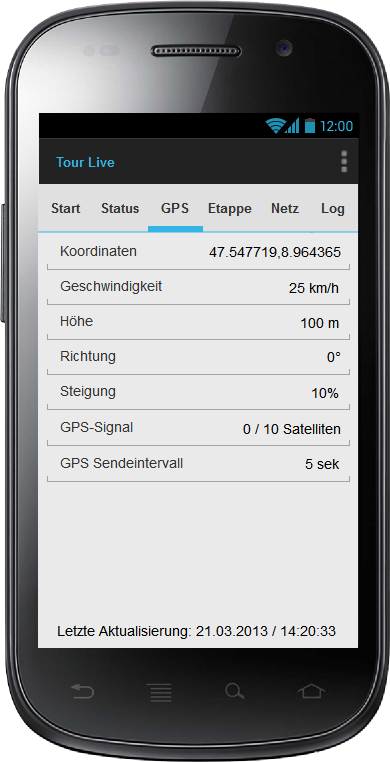
\includegraphics[width=4cm]{images/android/mockups/GPS.png} }
 &
\textbf{Erläuterung der Ansicht} \newline
\textbf{Koordinaten (*):} Empfangene GPS Koordinaten im Format WGS84\newline
\textbf{Geschwindigkeit (*):} Empfangene Geschwindigkeit vom Satellit gemessen\newline
\textbf{Höhe (*):} Höhe, vom Satellit ermittelt\newline
\textbf{Richtung (+):} Richtung in Grad, Abweichung von Norden, wichtig um zu erkennen, ob gleich wie die Windrichtung\newline
\textbf{Steigung (+):} Aktuelle Steigung über 100 Meter gemessen\newline
\textbf{GPS-Signal (*):} Verfügbarkeit der GPS-Satelliten\newline
\textbf{GPS-Intervall (°):} In welchem Intervall die GPS-Daten getracked werden. \newline
\textbf{Letzte Aktualisierung (*):} Zeitpunkt, der letzten Aktualisierung der Daten
\\

\end{longtable}

\subsubsection{Etappen – Übersicht}
Alle Informationen rund um die gesammelten Etappendaten.
\begin{longtable}{p{4cm} p{8cm}}
	\raisebox{-\totalheight}{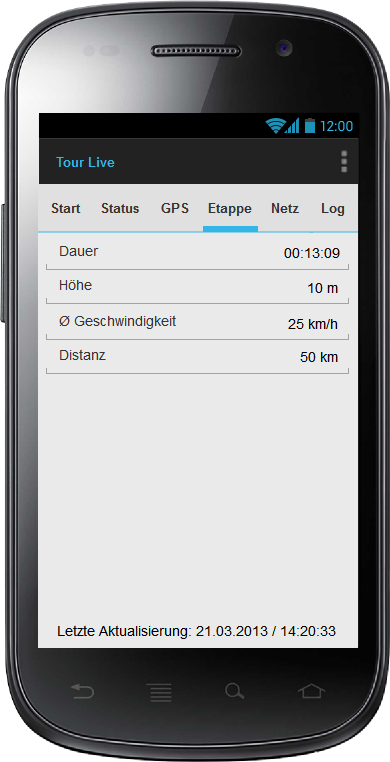
\includegraphics[width=4cm]{images/android/mockups/Etappe.png} }
 & 
\textbf{Erläuterung der Ansicht} \newline
\textbf{Dauer (*):} verstrichene Zeit während der aktuellen Etappe seitdem die Aufnahme gestartet wurde.\newline
\textbf{Höhe (*):} zurückgelegte Höhe, berechnet über alle bisher gesammelten Positionsdaten\newline
\textbf{Durchschnittsgeschwindigkeit (*):} Die Durchschnittliche Geschwindigkeit wird über alle der aktuellen Etappe gemessenen Positionsdaten ermittelt. \newline
\textbf{Distanz (*):} Die in der aktuellen Etappe zurückgelegten Kilometer. Wird ebenfalls über sämtliche der aktuellen Etappe ermittelten Positionsdaten berechnet.\newline
\textbf{Letzte Aktualisierung (+):} Zeitpunkt, der letzten Aktualisierung der Ansicht

\\

\end{longtable}


\subsubsection{Netz – Übersicht}
Folgende Ansicht dient zur Eruierung von Übertragungsproblemen. Zur anschliessenden Analyse der Qualität der Datenverbindung werden gleichzeitig zu den Positionsdaten auch Informationen zum vorhandenen Mobilfunknetzwerk gesammelt. 
\begin{longtable}{p{4cm} p{8cm}}
	\raisebox{-\totalheight}{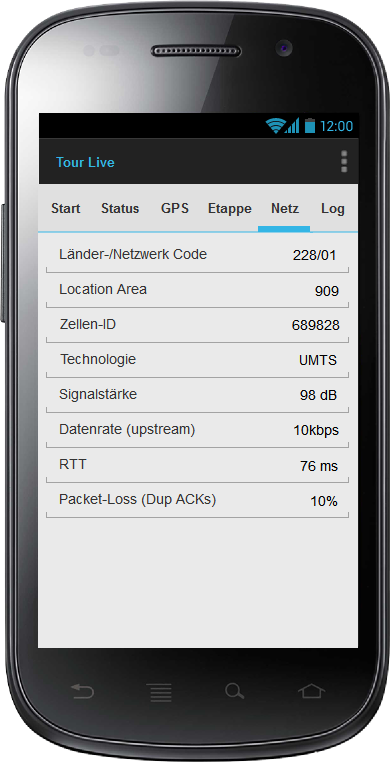
\includegraphics[width=4cm]{images/android/mockups/Netz.png} }
 & 
\textbf{Erläuterung der Ansicht} \newline
\textbf{Länder-/Netzwerk Code (+):} Mobile Country\footnote{Mobile Country Code, \url{http://en.wikipedia.org/wiki/Mobile_country_code}, aufgerufen am 22.03.2013} und Network Codes\footnote{Mobile Network Code, \url{http://en.wikipedia.org/wiki/Mobile_Network_Code},  aufgerufen am 22.03.2013}  \newline
\textbf{Location Area (+):} Eine Location-Area wird vom Mobilefunkanbieter definiert und fast mehrere Zellen (Antennen) zusammen.\newline
\textbf{Zellen-ID (+):} Zeigt die Zellennummer an mit der das Gerät aktuell verbunden ist.\newline
\textbf{Technologie (+):} Mobiles Kommunikationsprotokoll\newline
\textbf{Signalstärke (+):} Zeigt die aktuelle Mobilfunksignalstärke an\newline
\textbf{Datenrate (upstream) (+):} Gemessene Datenrate bei der Bildübertragung\newline
\textbf{RTT (+):} mit ICMP gemessene Round-Trip-Time\newline
\textbf{Packet-Loss (dup ACKs) (+):} Packetverlust beim Upload der Daten
\\

\end{longtable}




\subsubsection{Log }
Zur Fehlerbehebung allfälliger Fehler werden diverse Aktionen geloggt. 
\begin{longtable}{p{4cm} p{8cm}}
	\raisebox{-\totalheight}{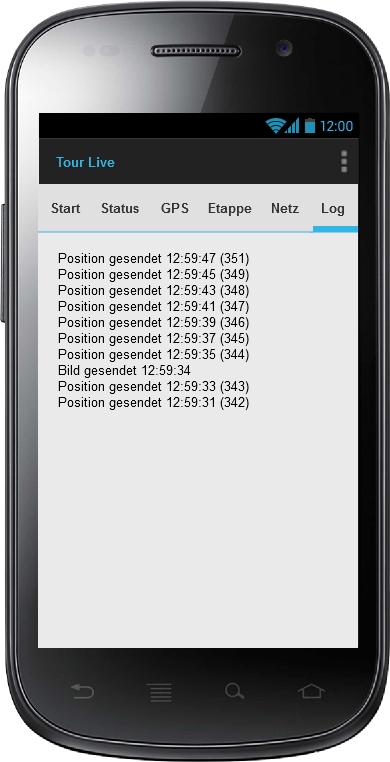
\includegraphics[width=4cm]{images/android/mockups/Log.png} }
 & 
Folgende Aktionen werden geloggt:
\begin{itemize}
\item Bild versendet
\item Daten versendet
\item Einstellungen synchronisiert
\item Aufgetrettene Exceptions
\end{itemize}
	

\\

\end{longtable}


\subsection{Einstellungen}
Über den „Settings“-Button in der rechten oberen Ecke werden die App-Einstellungen angepasst. Ist am Geräte ein physischer „Settings“-Knopf vorhanden, können die Einstellungen auch über diesen geöffnet werden.
\subsubsection{Nutzen / Zielperson}
Die Einstellungen werden entweder am Gerät (Betriebsmodus: unmanaged) oder über den DeviceManagementServer (Betriebsmodus: managed) vorgenommen. Die Einstellungen dienen vorgängig technisch versierten Personen um entsprechende Konfigurationen vorzunehmen. 

\begin{longtable}{p{4cm} p{8cm}}
	\raisebox{-\totalheight}{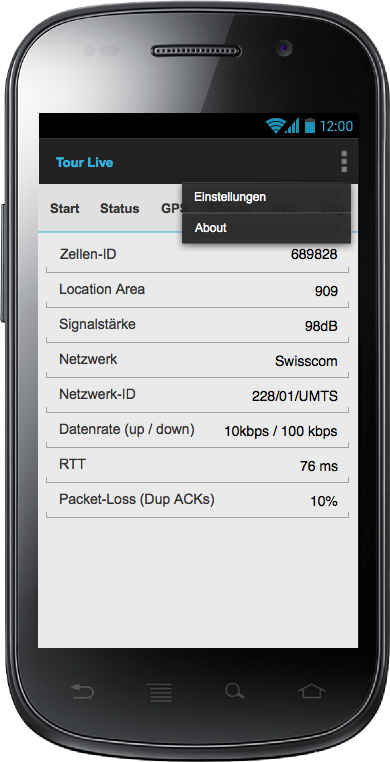
\includegraphics[width=4cm]{images/android/mockups/SettingsButtonPressed.png} }
 & 
\textbf{Erläuterung der Ansicht} \newline
\textbf{Einstellungen:} Einstellungen der App \newline
\textbf{About:} Zeigt den About Screen an
\end{longtable}

\begin{longtable}{p{4cm} p{8cm}}
	\raisebox{-\totalheight}{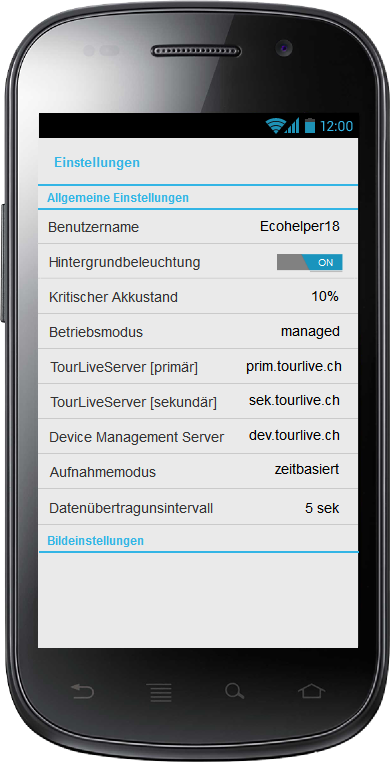
\includegraphics[width=4cm]{images/android/mockups/Einstellungen1.png} }
 & 
\textbf{Erläuterung der Ansicht} \newline
\textbf{Benutzername:} Benutzername zur Identifizierung des Gerätes für den Benutzer. Innerhalb des TourLiveSystems wird mit einer eindeutigen Geräteidentifikationsnummer gearbeitet \newline
\textbf{Hintergrundbeleuchtung:} Aktivierung / Deaktivierung der permanenten Hintergrundbeleuchtung  \newline
\textbf{Kritischer Akkustand:} Grenzwert „kritischer“ Akkuzustand für Power-Saving Funktionalität: nach Unterschreiten dieses Wertes werden Stromsparmassnahmen ergriffen \newline
\textbf{Betriebsmodus:} Betriebsmodus „managed“ oder „unmanaged“ \newline
\textbf{TourLiveServer [primär]:} Primärer TourLiveServer an den die Daten gesendet werden \newline
\textbf{TourLiveServer [sekundär]:} Sekundärer TourLiveServer der als Backup dient, falls der primäre TourLiveServer nicht mehr verfügbar ist  \newline
\textbf{Device Management Server:} Device Management Server mit dem die Gerätekonfiguration synchronisiert wird. \newline
\textbf{Aufnahmemodus:} Aufnahmemodus (zeitbasiert, manuell, fernsteuerung, aufgrund aktiver Stromzufuhr) \newline
\textbf{Datenübertragungsintervall:} Zeitintervall in dem die Positionsdaten/Netzwerkdaten aufgezeichnet, an den Server gesendet und die App-Views aktualisiert werden

\end{longtable}


\begin{longtable}{p{4cm} p{8cm}}
	\raisebox{-\totalheight}{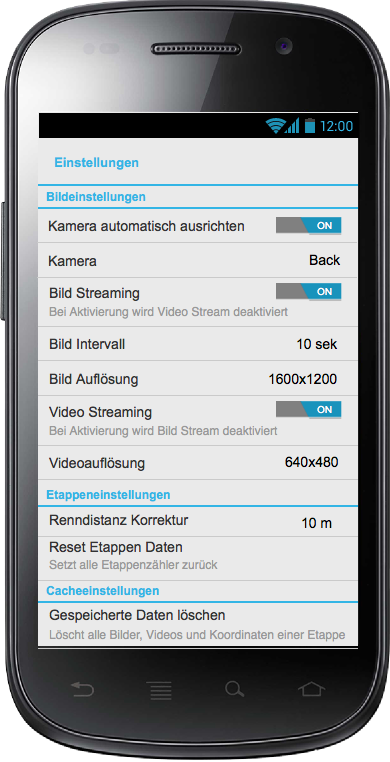
\includegraphics[width=4cm]{images/android/mockups/Einstellungen2.png} }
 & 
\textbf{Automatische Ausrichtung der Kamera:} Ist der „Switch“ deaktiviert, so kann über ein Untermenü die Ausrichtung der Kamera explizit definiert werden.\newline
\textbf{Bild- / Video - Streaming:} Aktivierung / Deaktivierung Übertragung von Bildern / Videos (es kann nur Video-Streaming oder Bilder-Streaming aktiv sein) \newline
\textbf{Kamera:} Zeigt die aktuelle Ausrichtung der Kamera an.\newline
\textbf{Bild Intervall:} Zeitintervall in dem die Bilder an den TourLive Server übertragen werden\newline
\textbf{Bild Auflösung:} Auflösung der Bilder (Abhängig vom Gerätetyp)\newline
\textbf{Video Streaming:} Aktivierung / Deaktivierung Übertragung vom Video-Stream (es kann nur Video-Streaming oder Bilder-Streaming aktiv sein)\newline
\textbf{Videoauflösung:} Auflösung des Video-Streams (Abhängig vom Kamera-Modell)

\end{longtable}
